\section{Core Path Algebra}

The core idea of the path algebra is to treat paths as first-class data objects, similar to tuples in relational algebra \cite{angles2024path}. The operators take sets of paths as input and return sets of paths, which allows their results to be combined into larger expressions.

\subsection{Core Operators}

The core algebra consists of three fundamental operators \cite{angles2024path}:

\begin{itemize}
    \item \textbf{Selection} ($\sigma$): filters paths based on predicates over node or edge labels and properties.
    \item \textbf{Union} ($\cup$): combines two sets of paths.
    \item \textbf{Concatenation (Join)} ($\bowtie$): concatenates paths whose endpoints are compatible.
\end{itemize}

%{
%\color{blue}


To illustrate these operators, we use the same running example throughout this section.

\begin{figure}[ht]
    \centering
    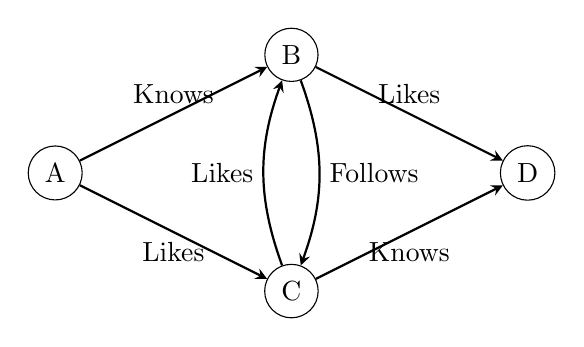
\begin{tikzpicture}[>=stealth]

        % Nodes
        \node[draw, circle] (A) at (0,0) {A};
        \node[draw, circle] (B) at (3,1.5) {B};
        \node[draw, circle] (C) at (3,-1.5) {C};
        \node[draw, circle] (D) at (6,0) {D};

        % Edges
        \draw[->, thick] (A) -- node[above] {Knows} (B);
        \draw[->, thick] (A) -- node[below] {Likes} (C);
        \draw[->, thick] (B) -- node[above] {Likes} (D);
        \draw[->, thick] (C) -- node[below] {Knows} (D);
        \draw[->, thick, bend left=20] (B) to node[right] {Follows} (C);
        \draw[->, thick, bend left=20] (C) to node[left] {Likes} (B);

    \end{tikzpicture}
    \caption{Example graph used throughout this section.}
\end{figure}

Assume the set $S$ contains all paths of length two starting from node $A$:

\[
p_1: A \rightarrow B \rightarrow D
\qquad
p_2: A \rightarrow C \rightarrow D
\qquad
p_3: A \rightarrow B \rightarrow C
\qquad
p_4: A \rightarrow C \rightarrow B
\]

%}
\subsection{Selection}
%{
%\color{blue}
Selection filters a set of paths according to predicates over nodes, edges, or their properties and is defined as follows:

\[
\sigma_c(S) = \{ p \in S \mid c(p) \}
\]

As an example, we filter the path set according to the label of the first edge.

\[
\sigma_{\text{Knows}}(S)=\{p_1,p_3\}
\]

\[
\sigma_{\text{Likes}}(S)=\{p_2,p_4\}
\]

The result is two subsets of $S$, each containing paths that satisfy the corresponding predicate. Unlike graph traversal itself, selection does not modify paths; it only filters the existing path set.
%}

\subsection{Union}
%{
%\color{blue}

Union combines two path sets into a single result.

Using the subsets obtained above,

\[
S_1=\sigma_{\text{Knows}}(S),
\qquad
S_2=\sigma_{\text{Likes}}(S),
\]

their union reconstructs the original path set:

\[
S_1\cup S_2
=
\{p_1,p_2,p_3,p_4\}
=
S.
\]

This illustrates that path sets from different query operations can be combined using the usual set-union semantics.

\subsection{Path Concatenation}
%{
%\color{blue}
Concatenation joins two compatible path fragments into a longer path. Two paths are compatible if the last node of the first path equals the first node of the second path.

Using the running example, we first consider shorter path fragments:

\[
A\rightarrow B,
\qquad
A\rightarrow C,
\]

and

\[
B\rightarrow D,
\qquad
C\rightarrow D.
\]

Concatenating compatible fragments produces longer paths:

\[
(A\rightarrow B)\circ(B\rightarrow D)
=
A\rightarrow B\rightarrow D
=
p_1,
\]

\[
(A\rightarrow C)\circ(C\rightarrow D)
=
A\rightarrow C\rightarrow D
=
p_2.
\]

A query can therefore construct longer paths from smaller path fragments. This is similar to a relational join, but the result is a path rather than a tuple.

\subsection{Closure and Compositionality}
%{
%\color{blue}
A central property of the core algebra is closure: every operator returns another set of paths. Consequently, the output of one operator can immediately serve as the input to another.

In the running example, the selection operator produced the path sets

\[
S_{\text{Knows}}
\quad\text{and}\quad
S_{\text{Likes}},
\]

which could subsequently be combined again using union or further extended using concatenation. Since every intermediate result remains a valid path set, complex path queries can be built from simpler expressions in a modular way.

This compositionality is one of the main strengths of the algebra. It allows query evaluation to be decomposed into reusable intermediate results, supports algebraic query optimization, and provides a clean logical foundation for graph query processing \cite{angles2024path}.
%}